\documentclass[11pt,addpoints,answers]{exam}

%-----------------------------------------------------------------------------
% PACKAGES AND OTHER DOCUMENT CONFIGURATIONS
%-----------------------------------------------------------------------------

\usepackage[margin=1in]{geometry}
\usepackage{amsmath, amsfonts}
\usepackage{enumerate}
\usepackage{graphicx}
\usepackage{titling}
\usepackage{url}
\usepackage{xfrac}
\usepackage{natbib}
\usepackage{amssymb}
\usepackage{amsthm}
\usepackage{paralist}
\usepackage{epstopdf}
\usepackage{tabularx}
\usepackage{longtable}
\usepackage{multirow}
\usepackage{multicol}
\usepackage[colorlinks=true,urlcolor=blue]{hyperref}
\usepackage{algorithm}
\usepackage{algorithmicx}
\usepackage[noend]{algpseudocode}
\usepackage{float}
\usepackage{enumerate}
\usepackage{array}
\usepackage{environ}
\usepackage{times}
\usepackage{textcomp}
\usepackage{caption}
\usepackage{parskip} % For NIPS style paragraphs.
\usepackage[compact]{titlesec} % Less whitespace around titles
\usepackage[inline]{enumitem} % For inline enumerate* and itemize*
\usepackage{datetime}
\usepackage{comment}
% \usepackage{minted}
\usepackage{lastpage}
\usepackage{color}
\usepackage{xcolor}
\usepackage[final]{listings}
\usepackage{tikz}
\usetikzlibrary{shapes,decorations}
\usepackage{framed}
\usepackage{booktabs}
\usepackage{cprotect}
\usepackage{verbatimbox}
\usepackage{multicol}
\usepackage{hyperref}
\usepackage{subcaption}
\usepackage{mathtools} % For drcases
\usepackage{cancel}
\usepackage[many]{tcolorbox}
\usepackage{soul}
\usepackage[bottom]{footmisc}
\usepackage{bm}
\usepackage{wasysym}

\usepackage{tikz}
\usetikzlibrary{shapes.geometric}
\usetikzlibrary{positioning, arrows, automata, calc}

\newtcolorbox[]{your_solution}[1][]{
    % breakable,
    enhanced,
    nobeforeafter,
    colback=white,
    title=Your Answer,
    sidebyside align=top,
    box align=top,
    #1
}

%%%%%%%%%%%%%%%%%%%%%%%%%%%%%%%%%%%%%%%%%%%
% Formatting for \CorrectChoice of "exam" %
%%%%%%%%%%%%%%%%%%%%%%%%%%%%%%%%%%%%%%%%%%%

\CorrectChoiceEmphasis{}
\checkedchar{\blackcircle}

%%%%%%%%%%%%%%%%%%%%%%%%%%%%%%%%%%%%%%%%%%%
% Rotated Column Headers                  %
%%%%%%%%%%%%%%%%%%%%%%%%%%%%%%%%%%%%%%%%%%%
\usepackage{adjustbox}
\usepackage{array}

%https://tex.stackexchange.com/questions/32683/rotated-column-titles-in-tabular

\newcolumntype{R}[2]{%
    >{\adjustbox{angle=#1,lap=\width-(#2)}\bgroup}%
    l%
    <{\egroup}%
}
\newcommand*\rot{\multicolumn{1}{R{45}{1em}}}% no optional argument here, please!


%%%%%%%%%%%%%%%%%%%%%%%%%%%%%%%%%%%%%%%%%%%
% Better numbering                        %
%%%%%%%%%%%%%%%%%%%%%%%%%%%%%%%%%%%%%%%%%%%

% \numberwithin{equation}{section} % Number equations within sections (i.e. 1.1, 1.2, 2.1, 2.2 instead of 1, 2, 3, 4)
% \numberwithin{figure}{section} % Number figures within sections (i.e. 1.1, 1.2, 2.1, 2.2 instead of 1, 2, 3, 4)
% \numberwithin{table}{section} % Number tables within sections (i.e. 1.1, 1.2, 2.1, 2.2 instead of 1, 2, 3, 4)

%%%%%%%%%%%%%%%%%%%%%%%%%%%%%%%%%%%%%%%%%%
% Custom commands                        %
%%%%%%%%%%%%%%%%%%%%%%%%%%%%%%%%%%%%%%%%%%

\newcommand{\vc}[1]{\boldsymbol{#1}}
\newcommand{\adj}[1]{\frac{d J}{d #1}}
\newcommand{\chain}[2]{\adj{#2} = \adj{#1}\frac{d #1}{d #2}}

\newcommand{\R}{\mathbb{R}}
\newcommand{\blackcircle}{\tikz\draw[black,fill=black] (0,0) circle (1ex);}
\renewcommand{\circle}{\tikz\draw[black] (0,0) circle (1ex);}

\newcommand{\emptysquare}{{\LARGE $\square$}\ \ }
\newcommand{\filledsquare}{{\LARGE $\boxtimes$}\ \ }
\newcommand{\emptycircle}{{\LARGE $\fullmoon$}\ \ }
\newcommand{\filledcircle}{{\LARGE $\newmoon$}\ \ }

\newcommand{\ntset}{test}

% mathcal
\newcommand{\Ac}{\mathcal{A}}
\newcommand{\Bc}{\mathcal{B}}
\newcommand{\Cc}{\mathcal{C}}
\newcommand{\Dc}{\mathcal{D}}
\newcommand{\Ec}{\mathcal{E}}
\newcommand{\Fc}{\mathcal{F}}
\newcommand{\Gc}{\mathcal{G}}
\newcommand{\Hc}{\mathcal{H}}
\newcommand{\Ic}{\mathcal{I}}
\newcommand{\Jc}{\mathcal{J}}
\newcommand{\Kc}{\mathcal{K}}
\newcommand{\Lc}{\mathcal{L}}
\newcommand{\Mc}{\mathcal{M}}
\newcommand{\Nc}{\mathcal{N}}
\newcommand{\Oc}{\mathcal{O}}
\newcommand{\Pc}{\mathcal{P}}
\newcommand{\Qc}{\mathcal{Q}}
\newcommand{\Rc}{\mathcal{R}}
\newcommand{\Sc}{\mathcal{S}}
\newcommand{\Tc}{\mathcal{T}}
\newcommand{\Uc}{\mathcal{U}}
\newcommand{\Vc}{\mathcal{V}}
\newcommand{\Wc}{\mathcal{W}}
\newcommand{\Xc}{\mathcal{X}}
\newcommand{\Yc}{\mathcal{Y}}
\newcommand{\Zc}{\mathcal{Z}}

% mathbb
\newcommand{\Ab}{\mathbb{A}}
\newcommand{\Bb}{\mathbb{B}}
\newcommand{\Cb}{\mathbb{C}}
\newcommand{\Db}{\mathbb{D}}
\newcommand{\Eb}{\mathbb{E}}
\newcommand{\Fb}{\mathbb{F}}
\newcommand{\Gb}{\mathbb{G}}
\newcommand{\Hb}{\mathbb{H}}
\newcommand{\Ib}{\mathbb{I}}
\newcommand{\Jb}{\mathbb{J}}
\newcommand{\Kb}{\mathbb{K}}
\newcommand{\Lb}{\mathbb{L}}
\newcommand{\Mb}{\mathbb{M}}
\newcommand{\Nb}{\mathbb{N}}
\newcommand{\Ob}{\mathbb{O}}
\newcommand{\Pb}{\mathbb{P}}
\newcommand{\Qb}{\mathbb{Q}}
\newcommand{\Rb}{\mathbb{R}}
\newcommand{\Sb}{\mathbb{S}}
\newcommand{\Tb}{\mathbb{T}}
\newcommand{\Ub}{\mathbb{U}}
\newcommand{\Vb}{\mathbb{V}}
\newcommand{\Wb}{\mathbb{W}}
\newcommand{\Xb}{\mathbb{X}}
\newcommand{\Yb}{\mathbb{Y}}
\newcommand{\Zb}{\mathbb{Z}}

% mathbf lowercase
\newcommand{\av}{\mathbf{a}}
\newcommand{\bv}{\mathbf{b}}
\newcommand{\cv}{\mathbf{c}}
\newcommand{\dv}{\mathbf{d}}
\newcommand{\ev}{\mathbf{e}}
\newcommand{\fv}{\mathbf{f}}
\newcommand{\gv}{\mathbf{g}}
\newcommand{\hv}{\mathbf{h}}
\newcommand{\iv}{\mathbf{i}}
\newcommand{\jv}{\mathbf{j}}
\newcommand{\kv}{\mathbf{k}}
\newcommand{\lv}{\mathbf{l}}
\newcommand{\mv}{\mathbf{m}}
\newcommand{\nv}{\mathbf{n}}
\newcommand{\ov}{\mathbf{o}}
\newcommand{\pv}{\mathbf{p}}
\newcommand{\qv}{\mathbf{q}}
\newcommand{\rv}{\mathbf{r}}
\newcommand{\sv}{\mathbf{s}}
\newcommand{\tv}{\mathbf{t}}
\newcommand{\uv}{\mathbf{u}}
\newcommand{\vv}{\mathbf{v}}
\newcommand{\wv}{\mathbf{w}}
\newcommand{\xv}{\mathbf{x}}
\newcommand{\yv}{\mathbf{y}}
\newcommand{\zv}{\mathbf{z}}

% mathbf uppercase
\newcommand{\Av}{\mathbf{A}}
\newcommand{\Bv}{\mathbf{B}}
\newcommand{\Cv}{\mathbf{C}}
\newcommand{\Dv}{\mathbf{D}}
\newcommand{\Ev}{\mathbf{E}}
\newcommand{\Fv}{\mathbf{F}}
\newcommand{\Gv}{\mathbf{G}}
\newcommand{\Hv}{\mathbf{H}}
\newcommand{\Iv}{\mathbf{I}}
\newcommand{\Jv}{\mathbf{J}}
\newcommand{\Kv}{\mathbf{K}}
\newcommand{\Lv}{\mathbf{L}}
\newcommand{\Mv}{\mathbf{M}}
\newcommand{\Nv}{\mathbf{N}}
\newcommand{\Ov}{\mathbf{O}}
\newcommand{\Pv}{\mathbf{P}}
\newcommand{\Qv}{\mathbf{Q}}
\newcommand{\Rv}{\mathbf{R}}
\newcommand{\Sv}{\mathbf{S}}
\newcommand{\Tv}{\mathbf{T}}
\newcommand{\Uv}{\mathbf{U}}
\newcommand{\Vv}{\mathbf{V}}
\newcommand{\Wv}{\mathbf{W}}
\newcommand{\Xv}{\mathbf{X}}
\newcommand{\Yv}{\mathbf{Y}}
\newcommand{\Zv}{\mathbf{Z}}

% bold greek lowercase
\newcommand{\alphav     }{\boldsymbol \alpha     }
\newcommand{\betav      }{\boldsymbol \beta      }
\newcommand{\gammav     }{\boldsymbol \gamma     }
\newcommand{\deltav     }{\boldsymbol \delta     }
\newcommand{\epsilonv   }{\boldsymbol \epsilon   }
\newcommand{\varepsilonv}{\boldsymbol \varepsilon}
\newcommand{\zetav      }{\boldsymbol \zeta      }
\newcommand{\etav       }{\boldsymbol \eta       }
\newcommand{\thetav     }{\boldsymbol \theta     }
\newcommand{\varthetav  }{\boldsymbol \vartheta  }
\newcommand{\iotav      }{\boldsymbol \iota      }
\newcommand{\kappav     }{\boldsymbol \kappa     }
\newcommand{\varkappav  }{\boldsymbol \varkappa  }
\newcommand{\lambdav    }{\boldsymbol \lambda    }
\newcommand{\muv        }{\boldsymbol \mu        }
\newcommand{\nuv        }{\boldsymbol \nu        }
\newcommand{\xiv        }{\boldsymbol \xi        }
\newcommand{\omicronv   }{\boldsymbol \omicron   }
\newcommand{\piv        }{\boldsymbol \pi        }
\newcommand{\varpiv     }{\boldsymbol \varpi     }
\newcommand{\rhov       }{\boldsymbol \rho       }
\newcommand{\varrhov    }{\boldsymbol \varrho    }
\newcommand{\sigmav     }{\boldsymbol \sigma     }
\newcommand{\varsigmav  }{\boldsymbol \varsigma  }
\newcommand{\tauv       }{\boldsymbol \tau       }
\newcommand{\upsilonv   }{\boldsymbol \upsilon   }
\newcommand{\phiv       }{\boldsymbol \phi       }
\newcommand{\varphiv    }{\boldsymbol \varphi    }
\newcommand{\chiv       }{\boldsymbol \chi       }
\newcommand{\psiv       }{\boldsymbol \psi       }
\newcommand{\omegav     }{\boldsymbol \omega     }

% bold greek uppercase
\newcommand{\Gammav     }{\boldsymbol \Gamma     }
\newcommand{\Deltav     }{\boldsymbol \Delta     }
\newcommand{\Thetav     }{\boldsymbol \Theta     }
\newcommand{\Lambdav    }{\boldsymbol \Lambda    }
\newcommand{\Xiv        }{\boldsymbol \Xi        }
\newcommand{\Piv        }{\boldsymbol \Pi        }
\newcommand{\Sigmav     }{\boldsymbol \Sigma     }
\newcommand{\Upsilonv   }{\boldsymbol \Upsilon   }
\newcommand{\Phiv       }{\boldsymbol \Phi       }
\newcommand{\Psiv       }{\boldsymbol \Psi       }
\newcommand{\Omegav     }{\boldsymbol \Omega     }

%%%%%%%%%%%%%%%%%%%%%%%%%%%%%%%%%%%%%%%%%%%
% Code highlighting with listings         %
%%%%%%%%%%%%%%%%%%%%%%%%%%%%%%%%%%%%%%%%%%%

\definecolor{bluekeywords}{rgb}{0.13,0.13,1}
\definecolor{greencomments}{rgb}{0,0.5,0}
\definecolor{redstrings}{rgb}{0.9,0,0}
\definecolor{light-gray}{gray}{0.95}

\newcommand{\MYhref}[3][blue]{\href{#2}{\color{#1}{#3}}}%

\definecolor{dkgreen}{rgb}{0,0.6,0}
\definecolor{gray}{rgb}{0.5,0.5,0.5}
\definecolor{mauve}{rgb}{0.58,0,0.82}

\lstdefinelanguage{Shell}{
  keywords={tar, cd, make},
  %keywordstyle=\color{bluekeywords}\bfseries,
  alsoletter={+},
  ndkeywords={python, py, javac, java, gcc, c, g++, cpp, .txt, octave, m, .tar},
  %ndkeywordstyle=\color{bluekeywords}\bfseries,
  identifierstyle=\color{black},
  sensitive=false,
  comment=[l]{//},
  morecomment=[s]{/*}{*/},
  commentstyle=\color{purple}\ttfamily,
  %stringstyle=\color{red}\ttfamily,
  morestring=[b]',
  morestring=[b]",
  backgroundcolor = \color{light-gray}
}

\lstset{columns=fixed, basicstyle=\ttfamily,
    backgroundcolor=\color{light-gray},xleftmargin=0.5cm,frame=tlbr,framesep=4pt,framerule=0pt}


%%%%%%%%%%%%%%%%%%%%%%%%%%%%%%%%%%%%%%%%%%%
% Custom box for highlights               %
%%%%%%%%%%%%%%%%%%%%%%%%%%%%%%%%%%%%%%%%%%%

% Define box and box title style
\tikzstyle{mybox} = [fill=blue!10, very thick,
    rectangle, rounded corners, inner sep=1em, inner ysep=1em]

% \newcommand{\notebox}[1]{
% \begin{tikzpicture}
% \node [mybox] (box){%
%     \begin{minipage}{\textwidth}
%     #1
%     \end{minipage}
% };
% \end{tikzpicture}%
% }

\NewEnviron{notebox}{

\begin{tikzpicture}
\node [mybox] (box){
    \begin{minipage}{\textwidth}
        \BODY
    \end{minipage}
};
\end{tikzpicture}
}

%%%%%%%%%%%%%%%%%%%%%%%%%%%%%%%%%%%%%%%%%%%
% Commands showing / hiding solutions     %
%%%%%%%%%%%%%%%%%%%%%%%%%%%%%%%%%%%%%%%%%%%

%% To HIDE SOLUTIONS (to post at the website for students), set this value to 0: 
\def\issoln{0}
% Some commands to allow solutions to be embedded in the assignment file.
\ifcsname issoln\endcsname \else \def\issoln{1} \fi
% Default to an empty solutions environ.
\NewEnviron{soln}{}{}
\if\issoln 1
% Otherwise, include solutions as below.
\RenewEnviron{soln}{
    \leavevmode\color{red}\ignorespaces
    % \textbf{Solution} \BODY
    \BODY
}{}
\fi

%% To HIDE TAGS set this value to 0:
\def\showtags{0}
%%%%%%%%%%%%%%%%
\ifcsname showtags\endcsname \else \def\showtags{1} \fi
% Default to an empty tags environ.
\NewEnviron{tags}{}{}
\if\showtags 1
% Otherwise, include solutions as below.
\RenewEnviron{tags}{
    \fbox{
    \leavevmode\color{blue}\ignorespaces
    \textbf{TAGS:} \texttt{\url{\BODY}}
    }
    \vspace{-.5em}
}{}
\fi

% Abhi messing around with examdoc
\qformat{\textbf{{\Large \thequestion \; \; \thequestiontitle \ (\totalpoints \ points)}} \hfill}
\renewcommand{\thequestion}{\arabic{question}}
\renewcommand{\questionlabel}{\thequestion.}

\renewcommand{\thepartno}{\arabic{partno}}
\renewcommand{\partlabel}{\thepartno.}
\renewcommand{\partshook}{\setlength{\leftmargin}{0pt}}

\renewcommand{\thesubpart}{\alph{subpart}}
\renewcommand{\subpartlabel}{(\thesubpart)}

\renewcommand{\thesubsubpart}{\roman{subsubpart}}
\renewcommand{\subsubpartlabel}{\thesubsubpart.}

% copied from stack overflow, as all good things are
\newcommand\invisiblesection[1]{%
  \refstepcounter{section}%
  \addcontentsline{toc}{section}{\protect\numberline{\thesection}#1}%
  \sectionmark{#1}}

% quite possibly the worst workaround i have made for this class
\newcommand{\sectionquestion}[1]{
\titledquestion{#1}
\invisiblesection{#1}
~\vspace{-1em}
}

%%%%%%%%%%%%%%%%%%%%%%%%%%%%%%%%%%%%%%%%%%%
% Commands for customizing the assignment %
%%%%%%%%%%%%%%%%%%%%%%%%%%%%%%%%%%%%%%%%%%%

\newcommand{\courseName}{10-301/10-601 Introduction to Machine Learning (Spring 2022)}
\newcommand{\hwName}{Homework 5: Neural Networks}
\newcommand{\dueDate}{2022-03-18}
\newcommand{\homeworktype}{\string programming}

\title{\textsc{\hwName}
%\thanks{Compiled on \today{} at \currenttime{}}
} % Title


\author{\courseName\\
\url{https://www.cs.cmu.edu/~mgormley/courses/10601/} \\
OUT: 2022-02-27 \\
DUE: \dueDate{} \\ 
TAs: Abbey, Abhi, Alex, Neural, Shelly, Udai
}

\date{}

%%%%%%%%%%%%%%%%%%%%%%%%%%%%%%%%%%%%%%%%%%%%%%%%%
% Useful commands for typesetting the questions %
%%%%%%%%%%%%%%%%%%%%%%%%%%%%%%%%%%%%%%%%%%%%%%%%%

\newcommand \expect {\mathbb{E}}
\newcommand \mle [1]{{\hat #1}^{\rm MLE}}
\newcommand \map [1]{{\hat #1}^{\rm MAP}}
\newcommand \argmax {\operatorname*{argmax}}
\newcommand \argmin {\operatorname*{argmin}}
\newcommand \code [1]{{\tt #1}}
\newcommand \datacount [1]{\#\{#1\}}
\newcommand \ind [1]{\mathbb{I}\{#1\}}

%%%%%%%%%%%%%%%%%%%%%%%%%%
% Document configuration %
%%%%%%%%%%%%%%%%%%%%%%%%%%

% Don't display a date in the title and remove the white space
\predate{}
\postdate{}
\date{}

% Don't display an author and remove the white space
%\preauthor{}
%\postauthor{}

%%%%%%%%%%%%%%%%%%
% Begin Document %
%%%%%%%%%%%%%%%%%% 

\begin{document}

\maketitle

\begin{notebox}
\paragraph{Summary} In this assignment, you will build an image recognition system using a neural network. In the Written component, you will walk through an on-paper example of how to implement a neural network. Then, in the Programming component, you will implement an end-to-end system that learns to perform image classification.
\end{notebox}
\newcommand \maxsubs {10 }
\section*{START HERE: Instructions}
\begin{itemize}

\item \textbf{Collaboration Policy}: Please read the collaboration policy here: \url{http://www.cs.cmu.edu/~mgormley/courses/10601/syllabus.html}

\item\textbf{Late Submission Policy:} See the late submission policy here: \url{http://www.cs.cmu.edu/~mgormley/courses/10601/syllabus.html}

\item\textbf{Submitting your work:} You will use Gradescope to submit
  answers to all questions\ifthenelse{\equal{\homeworktype}{\string written}}{}{ and code}. Please
  follow instructions at the end of this PDF to correctly submit all your code to Gradescope.

  \begin{itemize}
    
 % COMMENT IF NOT USING CANVAS
\begin{comment}
  \item \textbf{Canvas:} Canvas (\url{https://canvas.cmu.edu}) will be
    used for quiz-style problems (e.g. multiple choice, true / false,
    numerical answers). Grading is done automatically.
    %
    You may only \textbf{submit once} on canvas, so be sure of your
    answers before you submit. However, canvas allows you to work on
    your answers and then close out of the page and it will save your
    progress.  You will not be granted additional submissions, so
    please be confident of your solutions when you are submitting your
    assignment.
    %
    {\color{red} The above is true for future assignments, but this one
    allows {\bf unlimited submissions}.}
\end{comment}
    
  % COMMENT IF NOT USING GRADESCOPE
   \item \textbf{Written:} For written problems such as short answer, multiple choice, derivations, proofs, or plots, please use the provided template. Submissions can be handwritten onto the template, but should be labeled and clearly legible. If your writing is not legible, you will not be awarded marks. Alternatively, submissions can be written in LaTeX. Each derivation/proof should be completed in the boxes provided. You are responsible for ensuring that your submission contains exactly the same number of pages and the same alignment as our PDF template. If you do not follow the template, your assignment may not be graded correctly by our AI assisted grader.

  %   COMMENT IF NOT USING GRADESCOPE AUTOGRADER
  \ifthenelse{\equal{\homeworktype}{\string written}}{}{
\item \textbf{Programming:} You will submit your code for programming questions on the homework to Gradescope (\url{https://gradescope.com}). After uploading your code, our grading scripts will autograde your assignment by running your program on a virtual machine (VM). When you are developing, check that the version number of the programming language environment (e.g. Python 3.9.6) and versions of permitted libraries (e.g.  \texttt{numpy} 1.21.2 and \texttt{scipy} 1.7.1) match those used on Gradescope. You have \maxsubs free Gradescope programming submissions. After \maxsubs submissions, you will begin to lose points from your total programming score. We recommend debugging your implementation on your local machine (or the Linux servers) and making sure your code is running correctly first before submitting your code to Gradescope.}

  \end{itemize}
  
\ifthenelse{\equal{\homeworktype}{\string written}}{}{\item\textbf{Materials:} The data that you will need in order to complete this assignment is posted along with the writeup and template on the course website.}

\end{itemize}


%\ifthenelse{\equal{\homeworktype}{\string written}}{}{\begin{notebox}
%\paragraph{Linear Algebra Libraries} When implementing machine learning algorithms, it is often convenient to have a linear algebra library at your disposal. In this assignment, Java users may use EJML\footnote{\url{https://ejml.org}} or ND4J\footnote{\url{https://javadoc.io/doc/org.nd4j/nd4j-api/latest/index.html}} and C++ users may use Eigen\footnote{\url{http://eigen.tuxfamily.org/}}. Details below. 
%
%(As usual, Python users have NumPy.)
%
%\begin{description}
%\item[EJML for Java] EJML is a pure Java linear algebra package with three interfaces. We strongly recommend using the SimpleMatrix interface. The autograder will use EJML version 0.41. When compiling and running your code, we will add the additional command line argument {\footnotesize{\lstinline{-cp "linalg_lib/ejml-v0.41-libs/*:linalg_lib/nd4j-v1.0.0-M1.1-libs/*:./"}}}
%to ensure that all the EJML jars are on the classpath as well as your code. 

%\item[ND4J for Java] ND4J is a library for multidimensional tensors with an interface akin to Python's NumPy. The autograder will use ND4J version 1.0.0-M1.1. When compiling and running your code, we will add the additional command line argument {\footnotesize{\lstinline{-cp "linalg_lib/ejml-v0.41-libs/*:linalg_lib/nd4j-v1.0.0-M1.1-libs/*:./"}}} to ensure that all the ND4J jars are on the classpath as well as your code. 

%\item[Eigen for C++] Eigen is a header-only library, so there is no linking to worry about---just \lstinline{#include} whatever components you need. The autograder will use Eigen version 3.4.0. The command line arguments above demonstrate how we will call you code. When compiling your code we will include, the argument \lstinline{-I./linalg_lib} in order to include the \lstinline{linalg_lib/Eigen} subdirectory, which contains all the headers.

%\end{description} 
%We have included the correct versions of EJML/ND4J/Eigen in the \lstinline{linalg_lib.zip} posted on the Coursework page of the course website for your convenience. It contains the same \lstinline{linalg_lib/} directory that we will include in the current working directory when running your tests. Do {\bf not} include EJML, ND4J, or Eigen in your homework submission; the autograder will ensure that they are in place. 
%\end{notebox}}\clearpage

\section*{Instructions for Specific Problem Types}

For ``Select One" questions, please fill in the appropriate bubble completely:

\begin{quote}
\textbf{Select One:} Who taught this course?
    \begin{checkboxes}
     \CorrectChoice Matt Gormley
     \choice Marie Curie
     \choice Noam Chomsky
    \end{checkboxes}
\end{quote}

If you need to change your answer, you may cross out the previous answer and bubble in the new answer:

\begin{quote}
\textbf{Select One:} Who taught this course?
    {
    \begin{checkboxes}
     \CorrectChoice Matt Gormley
     \choice Marie Curie \checkboxchar{\xcancel{\blackcircle}{}}
     \choice Noam Chomsky
    \end{checkboxes}
    }
\end{quote}

For ``Select all that apply" questions, please fill in all appropriate squares completely:

\begin{quote}
\textbf{Select all that apply:} Which are scientists?
    {%
    \checkboxchar{$\Box$} \checkedchar{$\blacksquare$} % change checkbox style locally
    \begin{checkboxes}
    \CorrectChoice Stephen Hawking 
    \CorrectChoice Albert Einstein
    \CorrectChoice Isaac Newton
    \choice I don't know
    \end{checkboxes}
    }
\end{quote}

Again, if you need to change your answer, you may cross out the previous answer(s) and bubble in the new answer(s):

\begin{quote}
\textbf{Select all that apply:} Which are scientists?
    {%
    \checkboxchar{\xcancel{$\blacksquare$}} \checkedchar{$\blacksquare$} % change checkbox style locally
    \begin{checkboxes}
    \CorrectChoice Stephen Hawking 
    \CorrectChoice Albert Einstein
    \CorrectChoice Isaac Newton
    \choice I don't know
    \end{checkboxes}
    }
\end{quote}

For questions where you must fill in a blank, please make sure your final answer is fully included in the given space. You may cross out answers or parts of answers, but the final answer must still be within the given space.

\begin{quote}
\textbf{Fill in the blank:} What is the course number?

\begin{tcolorbox}[fit,height=1cm, width=4cm, blank, borderline={1pt}{-2pt},nobeforeafter]
    \begin{center}\huge10-601\end{center}
    \end{tcolorbox}\hspace{2cm}
    \begin{tcolorbox}[fit,height=1cm, width=4cm, blank, borderline={1pt}{-2pt},nobeforeafter]
    \begin{center}\huge10-\xcancel{6}301\end{center}
    \end{tcolorbox}
\end{quote}

\clearpage
\clearpage

{\LARGE \bf Written Questions (\numpoints \ points)} 
\begin{questions}
\sectionquestion{Example Feed Forward and Backpropagation}
\label{sec:onelayertoy}
\begin{figure}[h]
    \def\distH{3.6cm}
    \def\distHTwo{0.1cm}
    \def\distHThree{0.3cm}
    \def\distV{0.6cm}
    \def\distVTwo{0.3cm}
    \centering
    % \includegraphics[scale=0.8]{img/oneHL6.png}
    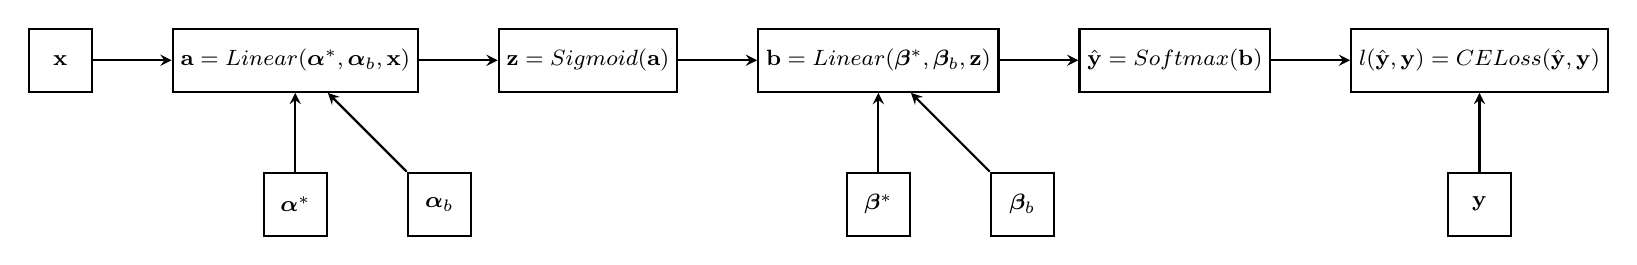
\begin{tikzpicture}[
            > = stealth, % arrow head style
            shorten > = 0pt, % don't touch arrow head to node
            auto,
            % node distance = 2.5cm, % distance between nodes
            thick % line style
        ]\footnotesize

        \tikzstyle{every state}=[
            draw = black,
            thick,
            fill = white,
            minimum size = 0.8cm,
            shape = rectangle
        ]
        \node[state] (X0) {$\xv$};
        \node[state] (a) [right = \distHThree of X0] {$\av = Linear(\alphav^*, \alphav_{b}, \xv)$};
        \node[state] (alpha1) [below = \distV of a] { $\alphav^*$};
        \node[state] (alpha0) [right = \distHTwo of alpha1] {$\alphav_{b}$};
        \node[state] (z) [right = \distHThree of a] {$\zv = Sigmoid(\av)$};
        \node[state] (b) [right = \distHThree of z] {$\bv = Linear(\betav^*,\betav_b, \zv)$};
        \node[state] (beta1) [below = \distV of b] {$\betav^*$};
        \node[state] (beta0) [right = \distHTwo of beta1] {$\betav_{b}$};
        \node[state] (y_hat) [right = \distHThree of b] {$\hat{\yv} = Softmax(\bv)$};
        \node[state] (loss) [right = \distHThree of y_hat] {$l(\hat{\yv},\yv) = CELoss(\hat{\yv},\yv)$};
        \node[state] (y) [below = \distV of loss] {$\yv$};
        \path[->] (X0) edge node {} (a);
        \path[->] (a) edge node {} (z);
        \path[->] (z) edge node {} (b);
        \path[->] (b) edge node {} (y_hat);
        \path[->] (y_hat) edge node {} (loss);
        \path[->] (alpha1) edge node {} (a);
        \path[->] (alpha0) edge node {} (a);
        \path[->] (beta1) edge node {} (b);
        \path[->] (beta0) edge node {} (b);
        \path[->] (y) edge node {} (loss);
        
        \begin{comment}
        \node[state] (X0) {$1$};
        \node[state] (X1) [below = \distV of X0] {$x_1$};
        \node[state] (X2) [below = \distV of X1] {$x_2$};
        \node[state] (X3) [below = \distV of X2] {$x_3$};
        \node[state] (X4) [below = \distV of X3] {$x_4$};
        \node[state] (X5) [below = \distV of X4] {$x_5$};
        \node[state] (X6) [below = \distV of X5] {$x_6$};
        \node[state] (A1) [right = \distH of X2] {$a_1$};
        \node[state] (A2) [below = \distV of A1] {$a_2$};
        \node[state] (A3) [below = \distV of A2] {$a_3$};
        \node[state] (A4) [below = \distV of A3] {$a_4$};
        \node[state] (Z1) [right = \distHTwo of A1] {$z_1$};
        \node[state] (Z2) [below = \distV of Z1] {$z_2$};
        \node[state] (Z3) [below = \distV of Z2] {$z_3$};
        \node[state] (Z4) [below = \distV of Z3] {$z_4$};
        \node[state] (Z0) [above = \distV of Z1] {$1$};
        \node[state] (B1) [below right = \distVTwo and \distH of A1] {$b_1$};
        \node[state] (B2) [below = \distV of B1] {$b_2$};
        \node[state] (B3) [below = \distV of B2] {$b_3$};
        \node[state] (Y1) [right = \distHThree of B1] {$\hat{y}_1$};
        \node[state] (Y2) [below = \distV of Y1] {$\hat{y}_2$};
        \node[state] (Y3) [below = \distV of Y2] {$\hat{y}_3$};
        \node[state] (l) [right = \distHThree of Y2] {$l$};

        \path[->] (X0) edge node {$\alpha_{1,0}$} (A1);
        \path[->] (X0) edge node {} (A2);
        \path[->] (X0) edge node {} (A3);
        \path[->] (X0) edge node {} (A4);
        \path[->] (X1) edge node {} (A1);
        \path[->] (X1) edge node {} (A2);
        \path[->] (X1) edge node {} (A3);
        \path[->] (X1) edge node {} (A4);
        \path[->] (X2) edge node {} (A1);
        \path[->] (X2) edge node {} (A2);
        \path[->] (X2) edge node {} (A3);
        \path[->] (X2) edge node {} (A4);
        \path[->] (X3) edge node {} (A1);
        \path[->] (X3) edge node {} (A2);
        \path[->] (X3) edge node {} (A3);
        \path[->] (X3) edge node {} (A4);
        \path[->] (X4) edge node {} (A1);
        \path[->] (X4) edge node {} (A2);
        \path[->] (X4) edge node {} (A3);
        \path[->] (X4) edge node {} (A4);
        \path[->] (X5) edge node {} (A1);
        \path[->] (X5) edge node {} (A2);
        \path[->] (X5) edge node {} (A3);
        \path[->] (X5) edge node {} (A4);
        \path[->] (X6) edge node {} (A1);
        \path[->] (X6) edge node {} (A2);
        \path[->] (X6) edge node {} (A3);
        \path[->] (X6) edge node {} (A4);
        \path[->] (Z0) edge node {$\beta_{1,0}$} (B1);
        \path[->] (Z0) edge node {} (B2);
        \path[->] (Z0) edge node {} (B3);
        \path[->] (Z1) edge node {} (B1);
        \path[->] (Z1) edge node {} (B2);
        \path[->] (Z1) edge node {} (B3);
        \path[->] (Z2) edge node {} (B1);
        \path[->] (Z2) edge node {} (B2);
        \path[->] (Z2) edge node {} (B3);
        \path[->] (Z3) edge node {} (B1);
        \path[->] (Z3) edge node {} (B2);
        \path[->] (Z3) edge node {} (B3);
        \path[->] (Z4) edge node {} (B1);
        \path[->] (Z4) edge node {} (B2);
        \path[->] (Z4) edge node {} (B3);
        \path[->] (B1) edge node {} (Y1);
        \path[->] (B1) edge node {} (Y2);
        \path[->] (B1) edge node {} (Y3);
        \path[->] (B2) edge node {} (Y1);
        \path[->] (B2) edge node {} (Y2);
        \path[->] (B2) edge node {} (Y3);
        \path[->] (B3) edge node {} (Y1);
        \path[->] (B3) edge node {} (Y2);
        \path[->] (B3) edge node {} (Y3);
        \path[->] (Y1) edge node {} (l);
        \path[->] (Y2) edge node {} (l);
        \path[->] (Y3) edge node {} (l);
        \path[->] (A1) edge node {} (Z1);
        \path[->] (A2) edge node {} (Z2);
        \path[->] (A3) edge node {} (Z3);
        \path[->] (A4) edge node {} (Z4);
        \end{comment}
    \end{tikzpicture}
    \caption{Computational Graph for a One Hidden Layer Neural Network}
    \label{fig:oneHL}
\end{figure}
\normalsize

\paragraph{Network Overview}
Consider the neural network with one hidden layer shown in Figure \ref{fig:oneHL}. The input layer consists of 6 features $\xv = [x_1,...,x_6]^T$, the hidden layer has 4  nodes $\zv = [z_1,...,z_4]^T$, and the output layer is a probability distribution $\yv = [y_1, y_2, y_3]^T$ over 3 classes (\textbf{1-indexed} such that $y_i$ is the probability of label $i$).

$\alphav^*$ is the matrix of weights from the inputs to the hidden layer and $\betav^*$ is the matrix of weights from the hidden layer to the output layer. 

$\alpha^*_{j,i}$ represents the weight going \textit{to} the node $z_j$ in the hidden layer \textit{from} the node $x_i$ in the input layer (e.g. $\alpha^*_{1,2}$ is the weight from $x_2$ to $z_1$), and $\betav^*$ is defined similarly. We will use a sigmoid activation function for the hidden layer and a softmax for the output layer.

The bias vectors $\alphav_b, \betav_b$ are defined such that the $j$th value of $\alphav_b$ (which we denote $\alpha_{j, b}$) is the bias value for $a_j$ and the $k$th value of $\betav_b$ is the bias value for $b_k$.

\paragraph{Network Details}

Equivalently, we define each of the following. 

The input:
\begin{align}
\label{eqn:x}
\xv=[x_1,x_2,x_3,x_4,x_5,x_6]^T
\end{align}

Linear combination at the first (hidden) layer:
\begin{equation}
\label{eqn:a}
a_j= \alpha_{j, b} + \sum_{i=1}^6 \alpha^*_{j,i}\cdot x_i,\,\, \forall j \in \{1,\ldots,4\}
\end{equation}

Activation at the first (hidden) layer:
\begin{align}
\label{eqn:z}
z_j &= \sigma(a_j) = \frac{1}{1+\exp(-a_j)},\,\, \forall j \in \{1,\ldots,4\}
\end{align}
Equivalently, we can write this as vector operation where the sigmoid activation is applied individually to each element of the vector $\av$:
\begin{align}
\label{eqn:zv}
\zv &= \sigma(\av)
\end{align}

Linear combination at the second (output) layer:
\begin{equation}
\label{eqn:b}
b_k = \beta_{k, b} + \sum_{j=1}^4 \beta^*_{k,j}\cdot z_j,\,\, \forall k \in \{1,\ldots,3\}
\end{equation}

Activation at the second (output) layer:
\begin{equation}
\label{eqn:yhat}
\hat{y}_k = \frac{\exp(b_k)}{\sum\limits_{l=1}^3 \exp(b_l)},\,\, \forall k \in \{1,\ldots,3\}
\end{equation}

\paragraph{Loss}

We will use cross entropy loss, $\ell(\hat{\yv},\yv)$. If $\yv$ represents our target output, which will be a one-hot vector representing the correct class, and $\hat{\yv}$ represents the output of the network, the loss is calculated by:
\begin{equation}
\label{eqn:loss}
  \ell(\hat{\yv},\yv) = - \sum_{i=1}^3 y_i \log(\hat{y}_i)
\end{equation}
{\bf For the below questions use natural log in the equation.} \\

\paragraph{Prediction}
When doing prediction, we will predict the $\argmax$ of the output layer. For example, if $\hat{y}_1=0.3, \hat{y}_2=0.2, \hat{y}_3=0.5$ we would predict class 3. If the true class from the training data was $2$ we would have a one-hot vector $\yv$ with values $y_1=0$, $y_2=1$, $y_3=0$.

\begin{parts}

\part In the following questions you will derive the matrix and vector forms of the previous equations which define our neural network. These are what you should hope to program in order to keep your program under the Gradescope time-out.\\
When working these out it is important to keep a note of the vector and matrix dimensions in order for you to easily identify what is and isn't a valid multiplication. Suppose you are given an training example: $\xv^{(1)}=[x_1,x_2,x_3,x_4,x_5,x_6]^T$ with \textbf{label class 2}, so $\yv^{(1)}=[0,1,0]^T$. We initialize the network weights as:
\begin{center}
$$\boldsymbol{\alpha^*}=
    \begin{bmatrix}
    \alpha_{1,1} & \alpha_{1,2} & \alpha_{1,3} & \alpha_{1,4} & \alpha_{1,5} & \alpha_{1,6} \\
    \alpha_{2,1} & \alpha_{2,2} & \alpha_{2,3} & \alpha_{2,4} & \alpha_{2,5} & \alpha_{2,6} \\
    \alpha_{3,1} & \alpha_{3,2} & \alpha_{3,3} & \alpha_{3,4} & \alpha_{3,5} & \alpha_{3,6} \\
    \alpha_{4,1} & \alpha_{4,2} & \alpha_{4,3} & \alpha_{4,4} & \alpha_{4,5} & \alpha_{4,6}
    \end{bmatrix}$$
    
$$\boldsymbol{\beta^*}=
    \begin{bmatrix}
    \beta_{1,1} & \beta_{1,2} & \beta_{1,3} & \beta_{1,4} \\
    \beta_{2,1} & \beta_{2,2} & \beta_{2,3} & \beta_{2,4} \\
    \beta_{3,1} & \beta_{3,2} & \beta_{3,3} & \beta_{3,4}
    \end{bmatrix}
$$
\end{center}
    
We want to also consider the bias term and the weights on the bias terms (${\alpha}_{j,b}$ and ${\beta}_{k,b})$. To account for these we can add them as a new column to the beginning of our initial weight matrices to represent biases, (e.g. $\alpha_{1, 0} = \alpha_{1, b}$).

$$\boldsymbol{\alpha}=
    \begin{bmatrix}
    \textcolor{blue}{\alpha_{1,0}} & \alpha_{1,1} & \alpha_{1,2} & \alpha_{1,3} & \alpha_{1,4} & \alpha_{1,5} & \alpha_{1,6} \\
    \textcolor{blue}{\alpha_{2,0}} & \alpha_{2,1} & \alpha_{2,2} & \alpha_{2,3} & \alpha_{2,4} & \alpha_{2,5} & \alpha_{2,6} \\
    \textcolor{blue}{\alpha_{3,0}} & \alpha_{3,1} & \alpha_{3,2} & \alpha_{3,3} & \alpha_{3,4} & \alpha_{3,5} & \alpha_{3,6} \\
    \textcolor{blue}{\alpha_{4,0}} & \alpha_{4,1} & \alpha_{4,2} & \alpha_{4,0} & \alpha_{4,4} & \alpha_{4,5} & \alpha_{4,6}
    \end{bmatrix}$$
    
$$\boldsymbol{\beta}=
    \begin{bmatrix}
    \textcolor{blue}{\beta_{1,0}} & \beta_{1,1} & \beta_{1,2} & \beta_{1,3} & \beta_{1,4} \\
    \textcolor{blue}{\beta_{2,0}} & \beta_{2,1} & \beta_{2,2} & \beta_{2,3} & \beta_{2,4} \\
    \textcolor{blue}{\beta_{3,0}} & \beta_{3,1} & \beta_{3,2} & \beta_{3,3} & \beta_{3,4}
    \end{bmatrix}$$

    We then add a corresponding new first dimension to our input vectors, always set to 1 ($x_0^{(i)} = 1$), so our input becomes: $$\xv^{(1)}=[\textcolor{blue}{1},x_1,x_2,x_3,x_4,x_5,x_6]^T$$
    
    
    \begin{subparts}
        \subpart[1] By examining the shapes of the initial weight matrices, how many neurons do we have in the first hidden layer of the neural network? Do not include the bias in your count.
        
        \begin{your_solution}[title=Answer,height=2cm,width=4cm]
        % YOUR ANSWER 
        \end{your_solution}
        
        \subpart[1] How many output neurons will our neural network have?
        
        \begin{your_solution}[title=Answer,height=2cm,width=4cm]
        % YOUR ANSWER 
        \end{your_solution}
        
        \subpart[1] What is the vector $\av$ whose elements are made up of the entries $a_j$ in Equation \ref{eqn:a} (using $x^{(1)}_i$ in place of $x_i$). Write your answer in terms of $\bm{\alpha}$ and $\xv^{(1)}$.
        
        \begin{your_solution}[title=Answer,height=2cm,width=4cm]
        % YOUR ANSWER 
        \end{your_solution}
        
        \clearpage
        
        \subpart[1] \textbf{Select all that apply:} We cannot take the matrix multiplication of our weights $\betav$ and the vector $\zv = [z_1, z_2, z_3, z_4]^T$ since they are not compatible shapes. Which of the following would allow us to take the matrix multiplication of $\betav$ and $\zv$ such that the entries of the vector $\bv = \boldsymbol{\beta}\zv$ are equivalent to the values of $b_k$ in Equation \ref{eqn:b}? 
        {\checkboxchar{$\Box$} \checkedchar{$\blacksquare$}
        \begin{checkboxes}
        % YOUR ANSWER
        % Change \choice to \CorrectChoice for the appropriate selection/selections 
        \choice A) Remove the last column of $\boldsymbol{\beta}$
        \choice B) Remove the first row of $\zv$
        \choice C) Append a value of 1 to be the first entry of $\zv$.
        \choice D) Append an additional column of 1's to be the first column of $\boldsymbol{\beta}$ 
        \choice E) Append a row of 1's to be the first row of $\boldsymbol{\beta}$ 
        \choice F) Take the transpose of $\boldsymbol{\beta}$
        \end{checkboxes}
        }
        
        
        \subpart[1] What are the entries of the output vector $\hat{\yv}$? Your answer should be written in terms of $b_1,b_2,b_3$.
        
        \begin{your_solution}[title=$\hat{\mathbf{y}}$,height=5cm,width=15cm]
        % YOUR ANSWER 
        \end{your_solution}
    \end{subparts}


\clearpage
\part We will now derive the matrix and vector forms for the backpropagation algorithm, for example 
$$\frac{\partial \ell}{\partial \alphav} = 
    \begin{bmatrix}
        \frac{\partial \ell}{\partial \alpha_{10}} & \frac{\partial \ell}{\partial \alpha_{11}} & \dots  & \frac{\partial \ell}{\partial \alpha_{16}} \\
        \frac{\partial \ell}{\partial \alpha_{20}} & \frac{\partial \ell}{\partial \alpha_{21}} & \dots  & \frac{\partial \ell}{\partial \alpha_{26}} \\
        \vdots      & \vdots      & \ddots & \vdots \\
        \frac{\partial \ell}{\partial \alpha_{40}} & \frac{\partial \ell}{\partial \alpha_{41}} & \dots  & \frac{\partial \ell}{\partial \alpha_{46}}
    \end{bmatrix}$$

The mathematics which you have to derive in this section jump significantly in difficulty, you should always be examining the shape of the matrices and vectors and making sure that you are comparing your matrix elements with calculations of individual derivatives to make sure they match (e.g., the element of the matrix $(\frac{\partial \ell}{\partial \boldsymbol{\alpha}})_{2,1}$ should be equal to $\frac{\partial \ell}{\partial \alpha_{2,1}}$  ). Recall that $\ell$ is our loss function defined in Equation \ref{eqn:loss}:

{\bf Note}: all vectors are column vectors (i.e. an n dimensional vector $v \in \mathbb{R}^{n \times 1}$). \textbf{Assume that all input vectors to linear layers have a bias term folded in, unless otherwise specified}. All partial derivatives should be written in \href{https://en.wikipedia.org/wiki/Matrix_calculus#Denominator-layout_notation}{denominator layout notation}. An example of denominator notation is that $\frac{\partial \ell}{\partial \beta} \in \mathbb{R}^{3 \times 5}$ because $\beta \in \mathbb{R}^{3 \times 5}$.
    
    
\begin{subparts}
    \subpart[1] What is the derivative $\frac{\partial \ell}{\partial \hat{y}_i}$, where $1 \leq i \leq 3$? Your answer should be in terms of $y_i$ and $\hat{y}_i$. Recall that we define the loss $\ell(\hat{y}, y)$ as follows (\textit{note: log is a natural log}):
    \begin{align}
        \ell(\hat{\yv},\yv) = - \sum_{i=1}^3 y_i \log(\hat{y}_i) \tag{\ref{eqn:loss}}
    \end{align}
    
    \begin{your_solution}[title=${\partial \ell}/{\partial \hat{y}_i}$, height=3cm, width=15cm]
    \end{your_solution}
    
    \subpart[1] Suppose we have $\hat{y} = [0.2, 0.7, 0.1]^T$ and $y$ = $[0, 1, 0]^T$. Compute the value of $\frac{\partial \ell}{\partial b_2}$. Use your answer from part (a), as well as the fact that the derivative of the softmax function with respect to $b_k$ is as follows:
    \begin{equation}
    \label{eqn:dydbk}
    \frac{\partial \hat{y}_l}{\partial b_k} = \hat{y}_l(\Ib[k=l]-\hat{y}_k)
    \end{equation}
    where $\Ib[k=l]$ is an indicator function such that if $k=l$ then it returns value 1 and 0 otherwise. Show your work below.
    \newline \newline
    HINT: Recall that $\frac{\partial \ell}{\partial b_k} = \sum_l \frac{\partial \ell}{\partial \hat{y}_l}\frac{\partial \hat{y}_l}{\partial b_k}$.
    
    \begin{your_solution}[title=${\partial \ell}/{\partial b_2}$, height=6cm, width=15cm]
    \end{your_solution}

    \subpart[3] Now, write the derivative $\frac{\partial \ell}{\partial b_k}$ in a smart way such that you do not need the indicator function in Equation \ref{eqn:dydbk}. Write your solutions in terms of $\hat{y}_k,y_k$. Show your work below.
    
    \begin{your_solution}[title=$\partial \ell / \partial b_k$,height=11cm,width=15cm]
    % YOUR ANSWER 
    \end{your_solution}
    
    \clearpage
    
    \subpart[1] What are the elements of the vector $\frac{\partial \ell}{\partial \bv}$? (Recall that  $\yv^{(1)}=[0,1,0]^T$)
    
    \begin{your_solution}[title=$\partial \ell/\partial \bv$,height=2.5cm,width=15cm]
    % YOUR ANSWER 
    \end{your_solution}
    
    \subpart[2] What is the derivative $\frac{\partial \ell}{\partial \betav}$? Your answer should be in terms of $\frac{\partial \ell}{\partial \bv}$ and $\zv$. 
    
    You should first consider a single entry in this matrix: $\frac{\partial \ell}{\partial \beta_{kj}}$.
    
    \begin{your_solution}[title=$\partial \ell/\partial \betav$,height=6cm,width=15cm]
    % YOUR ANSWER 
    \end{your_solution}
    
    
    \subpart[1] Explain in one short sentence why we use the matrix $\betav^*$ (the matrix $\betav$ without the first column of ones) when calculating the derivative matrix $\frac{\partial \ell}{\partial \alpha}$?
    
    
    \begin{your_solution}[title=Answer,height=3cm,width=15cm]
    % YOUR ANSWER 
    \end{your_solution}
    
    \clearpage

    \subpart[1] What is the derivative $\frac{\partial \ell}{\partial \zv}$ (\textbf{not including the bias term})? Your answer should be in terms of $\frac{\partial \ell}{\partial \bv}$ and $\betav^*$.
    
    \begin{your_solution}[title=$\partial \ell/\partial \zv$,height=6cm,width=15cm]
    % YOUR ANSWER 
    \end{your_solution}
    
    \subpart[1] What is the derivative $\frac{\partial \ell}{\partial a_j}$ in terms of $\frac{\partial \ell}{\partial z_j}$ and $z_j$?
    
    \begin{your_solution}[title=$\partial \ell/\partial a_j$,height=3cm,width=15cm]
    % YOUR ANSWER 
    \end{your_solution}
    

    \subpart[1] What is the matrix $\frac{\partial \ell}{\partial \boldsymbol{\alpha}}$? Your answer should be in terms of $\frac{\partial \ell}{\partial \av}$ and $\xv^{(1)}$.
    
    \begin{your_solution}[title=$\partial \ell/\partial \alphav$,height=6cm,width=15cm]
    % YOUR ANSWER 
    \end{your_solution}
    
\end{subparts}



\clearpage    

\part Now you will put these equations to use in an example with numerical values. \textbf{You should use the answers you get here to debug your code.} \\
You are given a training example $\xv^{(1)}=[1,0,1,1,0,1]^T$ with \textbf{label class 2}, so $\yv^{(1)}=[0,1,0]^T$. We initialize the network weights as:
\begin{center}
$$\boldsymbol{\alpha^*}=
    \begin{bmatrix}
    1 & 2 & 0 & -1 & 3 & 2 \\
    2 & 3 & 1 & 0 & 1 & 1 \\
    1 & 3 & 1 & 2 & -1 & 2 \\
    0 & 1 & 2 & 0 & 0 & 3
    \end{bmatrix}$$
    
$$\boldsymbol{\beta^*}=
    \begin{bmatrix}
    1 & 2 & 0 & 1 \\
    1 & -1 & 3 & 2 \\
    3 & 0 & -1 & 1
    \end{bmatrix}
$$
\end{center}
    
We want to also consider the bias term and the weights on the bias terms (${\alpha}_{j,b}$ and ${\beta}_{j,b})$. Lets say they are all initialized to 1. To account for this we can add a column of 1's to the beginning of our initial weight matrices. 

$$\boldsymbol{\alpha}=
    \begin{bmatrix}
    \textcolor{blue}{1} & 1 & 2 & 0 & -1 & 3 & 2\\
    \textcolor{blue}{1} & 2 & 3 & 1 & 0 & 1 & 1 \\
    \textcolor{blue}{1} & 1 & 3 & 1 & 2 & -1 & 2 \\
    \textcolor{blue}{1} & 0 & 1 & 2 & 0 & 0 & 3
    \end{bmatrix}$$
    
$$\boldsymbol{\beta}=
    \begin{bmatrix}
    \textcolor{blue}{1} & 1 & 2 & 0 & 1 \\
    \textcolor{blue}{1} & 1 & -1 & 3 & 2 \\
    \textcolor{blue}{1} & 3 & 0 & -1 & 1
    \end{bmatrix}
$$

And we can set our first value of our input vectors to always be 1 ($x_0^{(i)} = 1$), so our input becomes: $$\xv^{(1)}=[\textcolor{blue}{1},1,0,1,1,0,1]^T$$

 Using the initial weights, run the feed forward of the network over this example (rounding to 4 decimal places during the calculation) and then answer the following questions. 
 
 % Showing  your  work  in  these  questions  is  optional,  but  it is  recommended  to  help  us  understand  where  any misconceptions may occur.
%In your responses, round to four decimal places---if the answer is an integer you need not include trailing zeros. 
% NOT NEEDED: (Note: the superscript $(1)$ simply indicates that a value corresponds to using training example $x^{(1)}$)
\clearpage
\begin{subparts}
    \subpart[1] What is $a_1$?

    \begin{your_solution}[title=$a_1$,height=2cm,width=3cm]
    % YOUR ANSWER 
    \end{your_solution}
    \begin{your_solution}[title=Work,height=4cm,width=12cm]
    % YOUR ANSWER 
    \end{your_solution}


    
    \subpart[1] What is $z_1$?
    
    \begin{your_solution}[title=$z_1$,height=2cm,width=3cm]
    % YOUR ANSWER 
    \end{your_solution}
    \begin{your_solution}[title=Work,height=4cm,width=12cm]
    % YOUR ANSWER 
    \end{your_solution}
    
    

    \subpart[1] What is $b_2$?  We have computed $z_2$ = 0.9933, $z_3$ = 0.9991, $z_4$ = 0.9975 for you.
    
   \begin{your_solution}[title=$b_2$,height=2cm,width=3cm]
    % YOUR ANSWER 
    \end{your_solution}
    \begin{your_solution}[title=Work,height=4cm,width=12cm]
    % YOUR ANSWER 
    \end{your_solution}
    
    \clearpage
    
    \subpart[1] What is $\hat{y}_2$? We have computed $b_1 = 4.9367, b_3 = 3.8562$ for you.
    
    \begin{your_solution}[title=$\hat{y}_2$,height=2cm,width=3cm]
    % YOUR ANSWER 
    \end{your_solution}
    \begin{your_solution}[title=Work,height=4cm,width=12cm]
    % YOUR ANSWER 
    \end{your_solution}

    \subpart[1] Which class would we predict on this example? Your answer should just be an integer $\in \{1, 2, 3\}$.
    
    \begin{your_solution}[title=Class,height=2cm,width=3cm]
    % YOUR ANSWER 
    \end{your_solution}
    \begin{your_solution}[title=Work,height=4cm,width=12cm]
    % YOUR ANSWER 
    \end{your_solution}
    
    
    \subpart[1] What is the total loss on this example?
    
    \begin{your_solution}[title=Loss,height=2cm,width=3cm]
    % YOUR ANSWER 
    \end{your_solution}
    \begin{your_solution}[title=Work,height=4cm,width=12cm]
    % YOUR ANSWER 
    \end{your_solution}
    
    
\end{subparts}

\clearpage
    

\part Now use the results of the previous question to run backpropagation over the network and update the weights with \textbf{Stochastic Gradient Descent}. Use learning rate $\eta=1$. 
    
Do your backpropagation calculations rounding to 4 decimal places then answer the following questions: 

\begin{subparts}
    \subpart[1] What is the value of $\frac{\partial \ell}{\partial \beta_{1,0}}$?
    
    \begin{your_solution}[title=$\partial \ell/\partial \beta_{1,0}$,height=2cm,width=3cm]
    % YOUR ANSWER 
    \end{your_solution}
    \begin{your_solution}[title=Work,height=5cm,width=12cm]
    % YOUR ANSWER 
    \end{your_solution}
    
    
 
    \subpart[1] What is the updated value of the weight $\beta_{1,0}$?
    
    \begin{your_solution}[title=$\beta_{1,0}$,height=2cm,width=3cm]
    % YOUR ANSWER 
    \end{your_solution}
    \begin{your_solution}[title=Work,height=4cm,width=12cm]
    % YOUR ANSWER 
    \end{your_solution}
    
    
    
    \subpart[1] What is the value of $\frac{\partial \ell}{\partial \alpha_{3,2}}$?
    
    \begin{your_solution}[title=$\partial \ell / \partial \alpha_{3,2}$,height=2cm,width=3cm]
    % YOUR ANSWER 
    \end{your_solution}
    \begin{your_solution}[title=Work,height=5cm,width=12cm]
    % YOUR ANSWER 
    \end{your_solution}
    
        \clearpage

    \subpart[1] What is the updated value of the weight ${\alpha}_{3,2}$?
    
    \begin{your_solution}[title=${\alpha}_{3,2}$,height=2cm,width=3cm]
    % YOUR ANSWER 
    \end{your_solution}
    \begin{your_solution}[title=Work,height=5cm,width=12cm]
    % YOUR ANSWER 
    \end{your_solution}
    
    
    \subpart[2] What is the updated weight of the input layer bias term applied to $z_2$ (i.e. ${\alpha}_{2,0}$)?
    
    \begin{your_solution}[title=${\alpha}_{2,0}$,height=2cm,width=3cm]
    % YOUR ANSWER 
    \end{your_solution}
    \begin{your_solution}[title=Work,height=14cm,width=12cm]
    % YOUR ANSWER 
    \end{your_solution}
    

\end{subparts}

\end{parts}
\newpage
\sectionquestion{Empirical Questions}
\label{sec:interp}

The following questions should be completed after you work through the programming portion of this assignment. \textbf{For any plotting questions, you must title your graph, label your axes and provide units, and provide a legend in order to receive full credit.}

For these questions, \textbf{use the small dataset}. Use the following values for the hyperparameters unless otherwise specified:

\begin{center}
    \begin{tabular}{|c|c|}
        \hline
        \textbf{Parameter} & \textbf{Value} \\
        \hline
        Number of Hidden Units & 50 \\
        \hline
        Weight Initialization & {\sc Random} \\
        \hline
        Learning Rate & 0.01 \\
        \hline
    \end{tabular}
\end{center}

Please submit computer-generated plots for all parts. To get full credit, your plots must have a label for both axes with the value plotted on that axis, provide a legend labeling every line, and have a title.

\begin{parts}
\part Hidden Units


\begin{subparts}

\subpart[2] Train a single hidden layer neural network using the hyperparameters mentioned in the table above, except for the number of hidden units which should vary among 5, 20, 50, 100, and 200.  Run the optimization for 100 epochs each time.

Plot the average training cross-entropy (sum of the cross-entropy terms over the training dataset divided by the total number of training examples) on the y-axis vs number of hidden units on the x-axis. In the \textbf{same figure}, plot the average validation cross-entropy.
        
\begin{your_solution}[title=Avg. Train and Validation Cross-Entropy Loss,height=10cm,width=14.5cm]
% YOUR ANSWER 
\end{your_solution}

\clearpage


\subpart[2] Examine and comment on the the plots of training and validation cross-entropy. What problem arises with too few hidden units, and why does it happen? 

\begin{your_solution}[title=Answer,height=4cm,width=14.5cm]
% YOUR ANSWER 
\end{your_solution}


\subpart[2] In the handout folder, we provide \texttt{metrics\_sgd\_small.txt}, a text file with the validation cross-entropy loss values for SGD performed using 100 epochs, 50 hidden units, random init, and 0.01 learning rate. In the \textbf{same figure}, plot them against your validation results for SGD \textbf{with} Adagrad using the same set of parameters and the small dataset.

\begin{your_solution}[title=Avg. Validation Cross-Entropy Loss of SGD with and without AdaGrad, height=10cm,width=14.5cm]
% YOUR ANSWER 
\end{your_solution}

\subpart[2] Examine and compare the two results. What do you observe?

\begin{your_solution}[title=Answer,height=3cm,width=14.5cm]
% YOUR ANSWER 
\end{your_solution}


\end{subparts}

\part Learning Rate


\begin{subparts}
\subpart[6] Train a single hidden layer neural network using the hyperparameters mentioned in the table above, except for the learning rate which should vary among 0.1, 0.01, and 0.001. Run the optimization for 100 epochs each time.

Plot the average training cross-entropy on the y-axis vs the number of epochs on the x-axis for the mentioned learning rates. In the \textbf{same figure}, plot the average validation cross-entropy loss. Make a separate figure for each learning rate.


\begin{your_solution}[title=Plot LR 0.1,height=10cm,width=14.5cm]
% YOUR ANSWER 
\end{your_solution}

\begin{your_solution}[title=Plot LR 0.01,height=10cm,width=14.5cm]
% YOUR ANSWER 
\end{your_solution}

\begin{your_solution}[title=Plot LR 0.001,height=10cm,width=14.5cm]
% YOUR ANSWER 
\end{your_solution}

\clearpage


\subpart[2] Examine and comment on the plots of training and validation cross-entropy. Are there any learning rates for which convergence is not achieved? Are there any learning rates that exhibit other problems? If so, describe these issues and list the learning rates that cause them.

\begin{your_solution}[title=Answer,height=5cm,width=14.5cm]
% YOUR ANSWER 
\end{your_solution}

\end{subparts}

\part Weight Initialization


\begin{subparts}

\subpart[2]
For this exercise, you can work on any data set. Initialize $\alphav$ and $\betav$ to zero and print them out after the first few updates. For example, you may use the following command to begin:  
\begin{lstlisting}[language=Shell]
$ python neuralnet.py small_train.csv small_validation.csv \
small_train_out.labels small_validation_out.labels \
small_metrics_out.txt 1 4 2 0.1
\end{lstlisting}
Compare the values across rows and columns in $\alphav$ and $\betav$. Describe the observed behavior and how this may affect model capacity and convergence.


\begin{your_solution}[title=Answer,height=5cm,width=14.5cm]
% YOUR ANSWER 
\end{your_solution}

\end{subparts}

\end{parts}
\newpage
\end{questions}

{\LARGE \bf Programming (94 points)}

\begin{figure}[H]
    \centering
    \captionsetup{justification=centering, margin=2cm}
    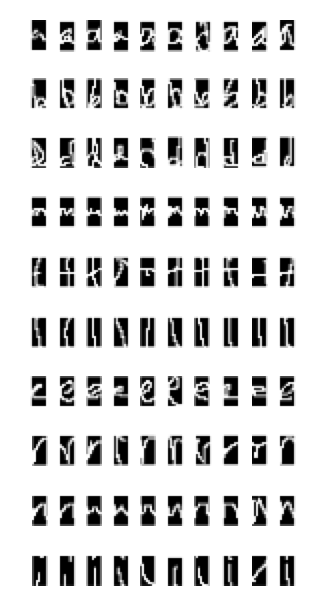
\includegraphics[scale=0.8]{img/lettergrid.png}
    \caption{10 random images of each of the 10 letters in the OCR dataset.}
    \label{fig:grid}
\end{figure}

\section{The Task}
Your goal in this assignment is to implement a neural network to classify images using a single hidden layer neural network. In addition, you will implement Adagrad, a variant of stochastic gradient descent. 

\section{The Datasets}
\label{sec:dataset}

\paragraph{Datasets} We will be using a subset of an Optical Character Recognition (OCR) dataset. This data includes images of all 26 handwritten letters; our subset will include only the letters ``a," ``e," ``g," ``i," ``l," ``n," ``o," ``r," ``t," and ``u."  The handout a small dataset with 60 samples \textit{per class} (50 for training and 10 for validation). We will also evaluate your code on a medium dataset with 600 samples per class (500 for training and 100 for validation). Figure \ref{fig:grid} shows a random sample of 10 images of few letters from the dataset.

% \paragraph{Datasets} We will be using a subset of a standard Computer Vision dataset, CIFAR-10. This data includes color images of various vehicles and animals; our subset will include black and white images of the 4 classes \verb|automobile|, \verb|bird|, \verb|frog|, \verb|ship|. The handout contains one dataset drawn from this data with 500 samples for training and 100 for validation.
% TODO: put sample of images in figure 4

\paragraph{File Format} Each dataset (small, medium, and large) consists of two csv files---train and validation. Each row contains 129 columns separated by commas. The first column contains the label and columns 2 to 129 represent the pixel values of a $16 \times 8$ image in a row major format. Label 0 corresponds to ``a," 1 to ``e," 2 to ``g," 3 to ``i," 4 to ``l," 5 to ``n," 6 to ``o," 7 to ``r," 8 to ``t," and 9 to ``u."

% \paragraph{File Format} Each dataset (small, medium, and large) consists of two csv files---train and validation. Each row contains 1025 columns separated by commas. The first column contains the label and columns 2 to 1025 represent the pixel values of a $32 \times 32$ image in a row major format. Label 0 corresponds to \verb|automobile|, 1 to \verb|bird|, 2 to \verb|frog|, and 3 to \verb|ship|.
%
Because the original images are black-and-white (not grayscale), the pixel values are either 0 or 1. However, you should write your code to accept arbitrary pixel values in the range [0, 1]. The images in Figure \ref{fig:grid} were produced by converting these pixel values into .png files for visualization. Observe that no feature engineering has been done here; instead the neural network you build will \emph{learn} features appropriate for the task of character recognition.

% You should write your code to accept arbitrary pixel values in the range [0, 1]. The images in Figure \ref{fig:grid} were produced by converting these pixel values into .png files for visualization. Observe that no feature engineering has been done here; instead the neural network you build will \emph{learn} features appropriate for the task of image recognition.


\section{Model Definition}
\label{sec:model}

In this assignment, you will implement a single-hidden-layer neural network with a sigmoid activation function for the hidden layer, and a softmax on the output layer. Let the input vectors $\xv$ be of length $M$, and the hidden layer $\zv$ consist of $D$ hidden units. In addition, let the output layer $\hat{\yv}$ be a probability distribution over $K$ classes. That is, each element $\hat{y}_k$ of the output vector represents the probability of $\xv$ belonging to the class $k$.

% \begin{align*}
% &  \hat{y}_k = \frac{\exp(b_k)}{\sum_{l=1}^K \exp(b_l)}
% \\
% & b_k =  \wv_2(k,0) + \sum_{j=1}^D \wv_2(k,j) z_j
% \\
% & z_j = \frac{1}{1+\exp(-a_j)}
% \\
% & a_j = \wv_1(j,0) + \sum_{m=1}^M \wv_1(j,m) x_m
% \end{align*}

We can compactly express this model by assuming that $x_0=1$ is a bias feature on the input and that $z_0=1$ is also fixed. In this way, we have two parameter matrices $\alphav \in \Rb^{D \times (M+1)}$ and $\betav \in \Rb^{K \times (D+1)}$. The extra $0$th column of each matrix (i.e. $\alphav_{\cdot, 0}$ and $\betav_{\cdot, 0}$) hold the bias parameters.

\begin{align*}
a_j &= \sum_{m=0}^M \alpha_{j,m} x_m
\\
z_j &= \frac{1}{1+\exp(-a_j)}
\\
b_k &= \sum_{j=0}^D \beta_{k,j} z_j
\\
\hat{y}_k &= \frac{\exp(b_k)}{\sum_{l=1}^K \exp(b_l)}
\\
\end{align*}

The objective function we will use for training the neural network is the average cross entropy over the training dataset $\Dc = \{ (\xv^{(i)}, \yv^{(i)}) \}$:

\begin{equation}
\label{eq:celoss}
J(\alphav, \betav)= - \frac{1}{N} \sum_{i=1}^N \sum_{k=1}^{K} y_k^{(i)} \log (\hat{y}^{(i)}_k)
\end{equation}

In Equation~\ref{eq:celoss}, $J$ is a function of the model parameters $\alphav$ and $\betav$ because $\hat{y}^{(i)}_k$ is implicitly a function of $\xv^{(i)}$, $\alphav$, and $\betav$ since it is the output of the neural network applied to $\xv^{(i)}$. $\hat{y}^{(i)}_k$ and $y_k^{(i)}$ are the $k$th components of $\hat{\yv}^{(i)}$ and $\yv^{(i)}$ respectively.

To train, you should optimize this objective function using stochastic gradient descent (SGD), where the gradient of the parameters for each training example is computed via backpropagation. You should shuffle the training points when performing SGD using the provided \verb|shuffle| function, passing in the epoch number as a random seed. Note that SGD has a slight impact on the objective function, where we are ``summing" over the current point, $i$:
\begin{equation}
\label{eq:sgd_celoss}
J_{SGD}(\alphav, \betav)= -\sum_{k=1}^{K} y_k^{(i)} \log (\hat{y}^{(i)}_k)
\end{equation}

Lastly, let's take a look at the Adagrad update that you will be performing. For each parameter $\theta^i_t$ at round $t$, you will first compute an intermediate value $\sv^i_t$, and then use this to compute the updated $\theta^i_{t+1}$.
$\sv^i_t$ will contain the element-wise sums (denoted by $\odot$) of all the element-wise squared gradients. Therefore, $\sv_t$ should have the same shape as $\frac{\partial J(\thetav_{t})}{\partial \thetav^i_t}$. $\sv_t$ should be initialized once, before the first epoch, to a zero vector. The update equations for $\sv$ and $\theta$ are below.

\begin{equation}
    \label{eq:adagrad_s}
    \sv^i_{t+1} = \sv^i_{t} + \frac{\partial J(\thetav_{t})}{\partial \thetav^i_t} \odot \frac{\partial J(\thetav_{t})}{\partial \thetav^i_t}.
\end{equation}

Then, we use $\sv_t$ to scale the gradient for the update:

\begin{equation}
    \label{eq:adagrad_update}
    \thetav^i_{t+1} = \thetav^i_t - \frac{\eta}{\sqrt{\sv^i_{t+1} + \epsilon}} \odot \frac{\partial J(\thetav_t)}{ \partial \thetav^i_t}.
\end{equation}

Here, $\eta$ is the learning rate, and $\epsilon =$ \texttt{1e-5}.

\subsection{Initialization}
\label{sec:init}

In order to use a deep network, we must first initialize the weights and biases in the network. This is typically done with a random initialization, or initializing the weights from some other training procedure. For this assignment, we will be using two possible initialization: 
\begin{quote}
\begin{description}
\item[{\sc Random}] The weights are initialized randomly from a uniform distribution from -0.1 to 0.1. The bias parameters are initialized to zero.
\item[{\sc Zero}] All weights are initialized to 0.  
\end{description}
\end{quote}

You must support both of these initialization schemes.

\section{Implementation}

Write a program \texttt{neuralnet.py} that implements an optical character recognizer using a one hidden layer neural network with sigmoid activations. Your program should learn the parameters of the model on the training data, report the cross-entropy at the end of each epoch on both train and validation data, and at the end of training write out its predictions and error rates on both datasets. 
%

Your implementation must satisfy the following requirements:

\begin{itemize}
    \item Use a {\bf sigmoid} activation function on the hidden layer and {\bf softmax} on the  output layer to ensure it forms a proper probability distribution.
    \item Number of {\bf hidden units} for the hidden layer should be determined by a command line flag.
    \item Support two different {\bf initialization strategies}, as described in Section \ref{sec:init}, selecting between them via a command line flag.
    \item Use stochastic gradient descent (SGD) to optimize the parameters for one hidden layer neural network. The number of {\bf epochs} will be specified as a command line flag. 
    \item Set the {\bf learning rate} via a command line flag.
    \item Perform stochastic gradient descent updates on the training data on the data shuffled with the provided function. For each epoch, you must reshuffle the \textbf{original} file data, not the data from the previous epoch.
    \item In case there is a tie in the output layer $\hat{\yv}$, predict the smallest index to be the label.
    \item You may assume that the input data will always have the same output label space (i.e. $\{0,1,\ldots,9\}$). Other than this, do not hard-code any aspect of the datasets into your code. We will autograde your programs on multiple data sets that include different examples.
    \item Do \emph{not} use any machine learning libraries. You may use NumPy.
\end{itemize}

Implementing a neural network can be tricky: the parameters are not just a simple vector, but a collection of many parameters; computational efficiency of the model itself becomes essential; the initialization strategy dramatically impacts overall learning quality;  other aspects which we will \emph{not} change (e.g. activation function, optimization method) also have a large effect. These \emph{tips} should help you along the way:

\begin{itemize}
\item Try to ``vectorize'' your code as much as possible---this is particularly important for Python. For example, in Python, you want to avoid for-loops and instead rely on \lstinline{numpy} calls to perform operations such as matrix multiplication, transpose, subtraction, etc. over an entire \lstinline{numpy} array at once. Why? Because these operations are actually implemented in fast C code, which won't get bogged down the way a high-level scripting language like Python will.
\item Implement a finite difference test to check whether your implementation of backpropagation is correctly computing gradients. If you choose to do this, comment out this functionality once your backward pass starts giving correct results and before submitting to Gradescope---since it will otherwise slow down your code.
\end{itemize}

\subsection{Command Line Arguments}
\label{sec:args}
The autograder runs and evaluates the output from the files generated, using the following command:

\begin{lstlisting}[language=Shell]
$ python3 neuralnet.py [args...]
\end{lstlisting}

Where above \texttt{[args\dots]} is a placeholder for nine command-line arguments: \texttt{<train\_input>}\newline \texttt{validation\_input> <train\_out> <validation\_out> <metrics\_out> <num\_epoch> \newline <hidden\_units>  <init\_flag> <learning\_rate>}. These arguments are described in detail below:
\begin{enumerate}
    \item \texttt{<train\_input>}: path to the training input \texttt{.csv} file (see Section~\ref{sec:dataset})
    \item \texttt{<validation\_input>}: path to the validation \ input \texttt{.csv} file (see Section~\ref{sec:dataset})
    \item \texttt{<train\_out>}: path to output \texttt{.labels} file to which the prediction on the \emph{training} data should be written (see Section~\ref{output})
    \item \texttt{<validation\_out>}: path to output \texttt{.labels} file to which the prediction on the \emph{validation} data should be written (see Section~\ref{output})
    \item \texttt{<metrics\_out>}: path of the output \texttt{.txt} file to which metrics such as train and validation\thinspace error should be written (see Section~\ref{metrics})
    \item \texttt{<num\_epoch>}: integer specifying the number of times backpropogation loops through all of the training data (e.g., if \texttt{<num\_epoch>} equals 5, then each training example will be used in backpropogation 5 times).
    \item \texttt{<hidden\_units>}: positive integer specifying the number of hidden units. 
    \item \texttt{<init\_flag>}: integer taking value 1 or 2 that specifies whether to use {\sc Random} or {\sc Zero} initialization (see Section~\ref{sec:init} and Section~\ref{sec:model})---that is, if \lstinline{init_flag}==1 initialize your weights randomly from a uniform distribution over the range [-0.1, 0.1] (i.e. {\sc Random}), if \lstinline{init_flag}==2 initialize all weights to zero (i.e. {\sc Zero}). For both settings, {\bf always initialize bias terms to zero}.
    \item \texttt{<learning\_rate>}: float value specifying the base learning rate for SGD with Adagrad.
     \item \texttt{<--debug>}: (optional argument) set the logging level, set to DEBUG to show logging
    
\end{enumerate}

As an example, if you implemented your program in Python, the following command line would run your program with 4 hidden units on the small data provided in the handout for 2 epochs using zero initialization and a learning rate of 0.1.
\\
\begin{lstlisting}[language=Shell]
python neuralnet.py small_train.csv small_validation.csv \
small_train_out.labels small_validation_out.labels \
small_metrics_out.txt 2 4 2 0.1 
\end{lstlisting}

\subsection{Output: Labels Files} \label{output}
Your program should write two output \texttt{.labels} files containing the predictions of your model on training data (\texttt{<train\_out>}) and validation\thinspace data (\texttt{<validation\_out>}). Each should contain the predicted labels for each example printed on a new line. Use \lstinline{\n} to create a new line. 

Your labels should exactly match those of a reference implementation -- this will be checked by the autograder by running your program and evaluating your output file against the reference solution.

\textbf{Note}: You should output your predicted labels using the same \emph{integer} identifiers as the original training data. You should also insert an empty line (again using ’\textbackslash n’) at the end of each sequence (as is done in the input data files).

\subsection{Debug Output: Logging}
Note that we use the debug logging level in the starter code.
If we use a higher logging level, we will log things with the default logging configuration, causing potential slowdowns when executing on an autograder.

Note also that we log NumPy matrices on separate lines from strings describing them. If we do not do this (e.g., if we call \verb|str| on them and add them to the strings), the arrays will be turned into strings even when our logging is set to ignore debug, causing potential massive slowdowns.

\subsection{Output Metrics} \label{metrics}
Generate a file where you report the following metrics: 

\begin{description}
\item[cross entropy] After each epoch, report mean cross entropy on the training data \lstinline{crossentropy(train)} and validation\thinspace data \texttt{crossentropy(validation)} (See Equation~\ref{eq:celoss}). These two cross-entropy values should be reported at the end of each epoch and prefixed by the epoch number. For example, after the second pass through the training examples, these should be prefixed by \lstinline{epoch=2}. The total number of train losses you print out should equal \texttt{num\_epoch}---likewise for the total number of validation\thinspace losses.
\item[error] After the final epoch (i.e. when training has completed fully), report the final training error \lstinline{error(train)} and validation\thinspace error \texttt{error(validation)}. 
\end{description}

%All of your reported numbers should be within 0.01 of the reference solution. 
A sample output is given below. It contains the train and validation\thinspace losses for the first 2 epochs and the final error rate when using the command given above.

\begin{lstlisting}
epoch=1 crossentropy(train): 1.9946950280285547
epoch=1 crossentropy(validation): 2.010686378337308
epoch=2 crossentropy(train): 1.912184059993547
epoch=2 crossentropy(validation): 1.944326942790059
error(train): 0.782
error(validation): 0.83
\end{lstlisting}

Take care that your output has the exact same format as shown above. There is an equal sign \lstinline{=} between the word \lstinline{epoch} and the epoch number, but no spaces. There should be a single space after the epoch number (e.g. a space after \lstinline{epoch=1}), and a single space after the colon preceding the metric value (e.g. a space after \lstinline{epoch=1 likelihood(train):}). Each line should be terminated by a Unix line ending \lstinline{\n}.

\subsection{Tiny Data Set} \label{tiny}
To help you with this assignment, we have also included a tiny data set, \texttt{tiny\_train.csv} and\\ \texttt{tiny\_validation.csv}, and a reference output file \texttt{tiny\_output.txt} for you to use. The tiny dataset is in a format similar to the other datasets, but it only contains two samples with five features. The reference file contains outputs from each layer of one correctly implemented neural network, for both forward and back-propagation steps. We advise you to use this set to help you debug in case your implementation doesn't produce the same results as in the written part.

For your reference, \texttt{tiny\_output.txt} is generated from the following command line specifications:

\begin{lstlisting}[language=Shell]
python neuralnet.py tiny_train.csv tiny_validation.csv \
tiny_train_out.labels tiny_validation_out.labels \
tiny_metrics_out.txt 1 4 2 0.1
\end{lstlisting}
The specific output file names are not important, but be sure to keep the other arguments exactly as they are shown above.

\section{Gradescope Submission}
You should submit your \texttt{neuralnet.py} to Gradescope. Please do not use any other file name for your implementation. This will cause problems for the autograder to correctly detect and run your code.

\section{Pseudocode}

Since the network structure we will use in this homework is fairly simple, we define our neural network as a single module. Note that in most deep learning libraries, there is a module corresponding to each layer type (e.g., Linear, Sigmoid, Softmax) to allow for more flexibility. We have provided more information about module-based programming in the additional readings in case you are interested.

\begin{description}
    \item{\textbf{NN Module}}
      \begin{algorithmic}[1]
        \Procedure{Forward}{$\xv$}
          \State Forward pass
        \EndProcedure
        \Procedure{Backward}{$\xv$,  $\yv$, $\hat{\yv}$}
          \State Backward pass
        \EndProcedure
        \Procedure{Train}{$\xv$, $\yv$}
            \State Train the model with SGD
        \EndProcedure
        \Procedure{Test}{$\xv$, $\yv$}
            \State Test the model and return the loss
        \EndProcedure
      \end{algorithmic}
\end{description}

The NN module defines a forward function $\yv = \textproc{Forward}(\xv)$ and a backward function $\gv_{\alpha}, \gv_{\beta} = \textproc{Backward}(\xv, \yv, \hat{\yv})$ method. You’ll want to pay close attention to the dimensions that you pass into and return from your modules.


\subsection{Forward and Backward Methods}

After implementing the helper functions (\textproc{SIGMOID}, \textproc{SOFTMAX}, \textproc{CROSSENTROPY}), we can define the methods \textproc{NNForward} and \textproc{NNBackward} as follows. 

\begin{algorithm}[H]
  \caption{Forward Method}
  \label{alg:forwardmodule}
  \begin{algorithmic}[1] % The number tells where the line numbering should start
    \Procedure{NNForward}{Training example ($\xv$, $\yv$)}
      \State $\av = \textproc{Linear}(\xv, \alphav)$
      \State $\zv = \textproc{Sigmoid}(\av)$
      \State $\bv = \textproc{Linear}(\zv, \betav)$
      \State $\hat{\yv} = \textproc{Softmax}(\bv)$
      \State \textbf{return} $\hat{\yv}$
    \EndProcedure
  \end{algorithmic}
\end{algorithm}

\begin{algorithm}[H]
  \caption{Backward Method}
  \label{alg:backpropmodule}
  \begin{algorithmic}[1] % The number tells where the line numbering should start
    \Procedure{NNBackward}{Training example ($\xv$, $\yv$), Predicted probabilities $\hat{\yv}$}
      \State Place intermediate quantities $\xv, \av, \zv, \bv, \hat{\yv}$ in scope \Comment{Hint: make use of class attributes}
      \State $\gv_{\bv} = \textproc{d\_CrossEntropy}(\yv, \hat{\yv})$
      \State $\gv_{\betav}, \gv_{\zv} = \textproc{d\_Linear}(\zv, \betav, \gv_{\bv})$
      \State $\gv_{\av} = \textproc{d\_Sigmoid}(\av, \zv) \gv_{\zv}$
      \State $\gv_{\alphav}, \gv_{\xv} = \textproc{d\_Linear
      }(\xv, \alphav, \gv_{\av})$ \Comment{We discard $\gv_{\xv}$}
      \State \textbf{return} parameter gradients $\gv_{\alphav}, \gv_{\betav}$
    \EndProcedure
  \end{algorithmic}
\end{algorithm}

\subsection{Training Method}
\label{sec:sgd}

% $\hat{\yv} = h_{\wv_1, \wv_2}(\xv) = \text{softmax}(\wv_2 \sigma(\wv_1 \xv + \wv_1_0) + \wv_2_0)$

Consider the neural network described in Section \ref{sec:model} applied to the $i$th training example $(\xv, \yv)$ where $\yv$ is a one-hot encoding of the true label. Our neural network outputs $\hat{\yv} = h_{\alphav, \betav}(\xv)$, where $\alphav$ and $\betav$ are the parameters of the first and second layers respectively and $h_{\alphav, \betav}$ is a one-hidden layer neural network with a sigmoid activation and softmax output. The loss function is negative cross-entropy $J = \ell(\hat{\yv}, \yv) = - \yv^T \log(\hat{\yv})$. $J = J_{\xv, \yv}(\alphav, \betav)$ is actually a function of our training example ($\xv, \yv$), and our model parameters $\alphav, \betav$ though we write just $J$ for brevity.

In order to train our neural network, we are going to apply stochastic gradient descent. Because we want the behavior of your program to be deterministic for testing on Gradescope, we make a few simplifications: (1) you should \emph{not} shuffle your data and (2) you will use a fixed learning rate. In the real world, you would \emph{not} make these simplifications. 

SGD proceeds as follows, where $E$ is the number of epochs and $\gamma$ is the learning rate.


\begin{algorithm}[H]
  \caption{Training with Stochastic Gradient Descent (SGD)}
  \label{alg:sgd}
  \begin{algorithmic}[1] % The number tells where the line numbering should start
    \Procedure{SGD}{Training data $\Dc_{train}$, \ntset\thinspace data $\Dc_t$} 
      \State Initialize parameters $\alphav, \betav$ \Comment{Use either {\sc Random} or {\sc Zero} from Section \ref{sec:init}}
      \For{$e \in \{1, 2, \ldots, E\}$} \Comment{For each epoch}
        \State $\Dc = \textproc{Shuffle}(\Dc_{train}, e)$
        \For{$(\xv, \yv) \in \Dc$} \Comment{For each training example (No shuffling)}
          \State Compute neural network layers:
          %$\hat{\yv} = h_{\wv_1, \wv_2}(\xv)$ and loss $J = \ell(\hat{\yv}, \yv)$ storing intermediate quantities as in 
          \State $\ov = \textproc{NNForward}(\xv, \yv, \alphav, \betav)$
          \State Compute gradients via backprop: 
            %    $\nabla_{\wv_1} J, \nabla_{\wv_2} J$
          %\State $\gv_{\wv_1} = \nabla_{\wv_1} J$
          %\State $\gv_{\wv_2} = \nabla_{\wv_2} J$ 
          \State 
              $
                \begin{drcases}
                \gv_{\alphav} = \frac{\partial J}{\partial \alphav} \\
                \gv_{\betav} = \frac{\partial J}{\partial \betav}
                \end{drcases} 
                = \textproc{NNBackward}(\xv, \yv, \hat{\yv})
              $
          \State Update parameters with Adagrad updates $\gv'_{\alphav}, \gv'_{\betav}$: \Comment{Refer to Eq.\ref{eq:adagrad_s}}
          \State $\alphav \gets \alphav - \gamma \gv'_{\alphav}$
          \State $\betav \gets \betav - \gamma \gv'_{\betav}$
            %   \State Update parameters:
            %   \State $\wv_1 \gets \wv_1 - \gamma \nabla_{\wv_1} J$ 
            %   \State $\wv_2 \gets \wv_2 - \gamma \nabla_{\wv_2} J$ 
        \EndFor
        \State Evaluate training mean cross-entropy $J_{\Dc}(\alphav, \betav)$
        \State Evaluate \ntset\thinspace mean cross-entropy $J_{\Dc_t}(\alphav, \betav)$
      \EndFor
      \State \textbf{return} parameters $\alphav, \betav$
    \EndProcedure
  \end{algorithmic}
\end{algorithm}

\subsection{Testing Method}
At test time, we output the most likely prediction for each example: 

\begin{algorithm}[H]
  \caption{Prediction at Test Time}
  \label{alg:predict}
  \begin{algorithmic}[1] % The number tells where the line numbering should start
    \Procedure{Predict}{Unlabeled train or \ntset\thinspace dataset $\Dc'$} 
    \For{$\xv \in \Dc'$}
      \State Compute neural network prediction $\hat{\yv} = h(\xv)$
      \State Predict the label with highest probability $l = \argmax_k \hat{y}_k$
    \EndFor
    \EndProcedure
  \end{algorithmic}
\end{algorithm}


% The dimensions $A$ and $B$ are specific to the module such that we have input $\av \in \Rb^A$, output $\bv \in \Rb^B$, gradient of output $\gv_{\av} \triangleq \nabla_{\av}J \in \Rb^A$, and gradient of input $\gv_{\bv} \triangleq \nabla_{\bv}J \in \Rb^B$. We have provided you the pseudocode for the Linear Module as an example.



It's also quite common to combine the Cross-Entropy and Softmax layers into one. The reason for this is the cancelation of numerous terms that result from the zeros in the cross-entropy backward calculation. (Said trick is \emph{not} required to obtain a sufficiently fast implementation for Gradescope.)
%You can read more about this in a detailed writeup from your TAs on Piazza.\footnote{\url{https://piazza.com/class/jar95m88puk3v6?cid=1092}} (Said trick is \emph{not} required to obtain a sufficiently fast implementation for Gradescope.)


Some additional tips: Make sure to read the autograder output carefully. The autograder for Gradescope prints out some additional 
information about the tests that it ran. For this programming assignment we've specially designed some buggy implementations that you might implement and will try our best to detect those and give you some more useful feedback in Gradescope's autograder. Make wise use of autograder's output for debugging your code.

Note: For this assignment, you may make up to 10 submissions to Gradescope before the deadline, but only your last submission will be graded.
\newpage

\newpage
\section{Collaboration Questions}
After you have completed all other components of this assignment, report your answers to these questions regarding the collaboration policy. Details of the policy can be found \href{http://www.cs.cmu.edu/~mgormley/courses/10601/syllabus.html}{here}.
\begin{enumerate}
    \item Did you receive any help whatsoever from anyone in solving this assignment? If so, include full details.
    \item Did you give any help whatsoever to anyone in solving this assignment? If so, include full details.
    \item Did you find or come across code that implements any part of this assignment? If so, include full details.
\end{enumerate}

\begin{your_solution}[height=6cm]
% YOUR ANSWER 

\end{your_solution}
\newpage

% \appendix
% \input{appendix.tex}

\end{document}